\newpage
\section[Herausforderungen bei der Implementierung von kryptografischen Funktionen in Webanwendungen]{Herausforderungen bei der Implementierung von \glsdisp{kryptografie}{kryptografischen} Funktionen in Webanwendungen}\label{sec:Herausforderung-bei-der-implementierung-von-kryptografie-in-webanwendungen}
In vielen Fällen überwiegt der Schutz, den \glsdisp{kryptografie}{kryptografische} Methoden bieten, den Aufwand und die Probleme, die bei der Implementierung auftreten.
Dennoch wird versucht, die Probleme, wie \zb die in \autoref{subsec:performance-und-skalierbarkeitsprobleme} beschriebenen Leistungseinbußen oder die in \autoref{subsec:benutzerfreundlichkeit_und_usability-aspekte} erläuterte erschwerte Benutzbarkeit, zu beheben, \bzw auf ein Minimum zu reduzieren.

\subsection[Performance- und Skalierbarkeitsprobleme]{Performance- und Skalierbarkeitsprobleme}\label{subsec:performance-und-skalierbarkeitsprobleme}
Der in \autoref{subsubsec:HTTPS-Protocol} vorgestellte Vorteil der verschlüsselten Übertragung bringt auch einen Nachteil mit sich.
Die Verschlüsselung der Daten verringert die Übertragungsrate und verlängert die Latenz der Übertragung\autocite[\pagef 5]{goldberg-comparison-nodate}, dies wird in \autoref{tab:HTTPS}\autocite[Übersetzt nach:][\pagef 5]{goldberg-comparison-nodate} dargestellt.

Diese Daten wurden vor 25 Jahren erfasst und seitdem ist \ac{HTTPS} verbessert, wodurch der nötige Performanceaufwand um eine verschlüsselte Verbindung aufzubauen, verringert wurde.\autocite[\vglf][]{CloudfareWarumHTTPS:online}

Neuere Versionen des \ac{TLS}\nonbreakdash \gls{algorithmus} bringen noch deutlichere Performance-Verbesserungen mit sich, da \uam nur ein \ac{TLS}-\gls{handshake}, vorgestellt auf Seite\ \pageref{par:tls_handshake_protocol}, benötigt wird, bzw.\ keiner, wenn bereits eine Verbindung zwischen \gls{client} und \gls{server} bestand\autocite[\vglf][]{CloudfareWarumHTTPS:online}.

\begin{table}[htpb]
    \caption[Parameter linearer Anpassungen an HTTP- und HTTPS-Übertragungen]{Parameter linearer Anpassungen an HTTP- und HTTPS-Übertragungen\footnotemark}
    \label{tab:HTTPS}
    \resizebox{0.9\textwidth}{!}{%
        \begin{tabular}{l|ll|ll}
            & \multicolumn{2}{l|}{Transferrate (bytes/ms)} & \multicolumn{2}{l}{Latenz (ms)} \\ \cline{2-5}
            Server        & Netscape & Mircosoft & Netscape & Microsoft \\ \hline
            Unsicher      & 946      & 829       & 4.5      & 19.0      \\
            \begin{tabular}[c]{@{}l@{}}
                Sicher \\ 40 bit
            \end{tabular} & 730      & 689       & 3.6      & 3.9       \\
            \begin{tabular}[c]{@{}l@{}}
                Sicher\\ 128 bit
            \end{tabular} & 736      & 686       & 25.0     & 5.1       \\ \hline
        \end{tabular}%
    }
\end{table}\ \footnotetext{\cite[\pagef 5]{goldberg-comparison-nodate}}

Gleichermaßen ist, trotz des Verdoppelns von CPU Geschwindigkeiten alle 18 Monate, die Performance von \ac{SSL} Maschinen noch immer ein Problem.\autocite[\vglf][\pagef 2]{cryptoeprint:2006/212}

%Wie \autoref{fig:reverse_ssl_handshake}\autocite[\pagef 3]{cryptoeprint:2006/212}  es darstellt, ist eine Möglichkeit, dies zu umgehen, das Entschlüsseln und Verifizieren des Zertifikates und der Signatur um die Identität des \glsdisp{client}{Clients} zu \glsdisp{authentifizierung}{authentifizieren}, die Kommunikationsrichtung der \glspl{handshake} umzukehren, also das Verifizieren und Entschlüsseln der Daten \glsdisp{server}{Serverside} anstatt \glsdisp{client}{Clientside} zu berechnen\autocite[\vglf][\pagef 3]{cryptoeprint:2006/212}
Gemäß \autoref{fig:reverse_ssl_handshake}\autocite[\pagef 3]{cryptoeprint:2006/212} kann die \gls{authentifizierung} der \gls{client}\nonbreakdash Identität durch Entschlüsselung und Verifizierung des Zertifikats und der Signatur erfolgen.
Eine Möglichkeit, dies zu erreichen, besteht darin, die Kommunikationsrichtung der \glspl{handshake} umzukehren.
Dies bedeutet, dass die Daten nun serverside anstatt clientside verifiziert und entschlüsselt werden.\autocite[\vglf][\pagef 2]{cryptoeprint:2006/212}
\begin{figure}[htpb]
    \centering
    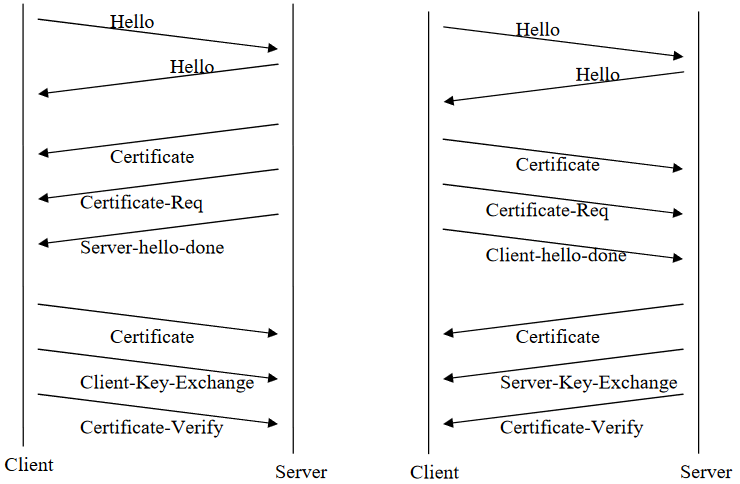
\includegraphics[width=0.75\linewidth]{abbildungen/reverse_ssl_handshake}
    \caption[Gegenüberstellung zwischen einem normalen SSL-Handshake (links) und einem umgekehrten SSL-Handshake (rechts)]{Gegenüberstellung zwischen einem normalen \ac{SSL}\nonbreakdash\gls{handshake} (links) und einem umgekehrten \ac{SSL}\nonbreakdash\gls{handshake} (rechts)\footnotemark}
    \label{fig:reverse_ssl_handshake}
\end{figure}~\footnotetext{\cite[\pagef 3]{cryptoeprint:2006/212}}

Da ein Großteil der Berechnungen für einen \ac{TLS}-\gls{handshake} während des Verifizierens der Zertifikate durchgeführt werden, wird die Laufzeit des \glspl{handshake} verbessert, wenn diese Berechnungen vom \gls{server} durchgeführt werden.

\subsection[Komplexität und Fehleranfälligkeit der Kryptografischen Methoden]{Komplexität und Fehleranfälligkeit der \glsdisp{kryptografie}{kryptografischen} Methoden}\label{subsec:komplexitaet_und_fehleranfaelligkeit_der_kryptografie}

\subsubsection[Komplexität bei der Implementierung von kryptografischen Methoden]{Komplexität bei der Implementierung von \glsdisp{kryptografie}{kryptografischen} Methoden in Webanwendungen}\label{subsubsec:komplexitaet_bei_der_implementierung_von_Kryptografischen_methoden_in_webanwendungen}
Durch die Vielzahl an Lektüre zu den verschiedenen Verschlüsselungsmethoden\autocites[\zb][]{davies2011implementing} ist es heutzutage nicht mehr so kompliziert, \glsdisp{kryptografie}{kryptografische} Methoden in Webanwendungen einzubauen, um Daten und die Anwendung als Ganzes zu sichern.
Für viele Programmiersprachen sind heutzutage vorgefertigte Methoden oder Packages entwickelt worden, welche verschiedene \glsdisp{kryptografie}{kryptografische} Methoden bereitstellen oder bündeln.
So stellt die Programmiersprache \ac{JS} die Funktion \lstinline!digest(algorithm, data)! zur Verfügung, welche einen Datensatz nach einem \ac{SHA}-\gls{algorithmus}\footnote{\ac{SHA}-1, \gls{SHA256}, \ac{SHA}-384 oder \ac{SHA}-512} verschlüsselt.\autocite[\vglf][]{SubtleCr83:online}
Die Funktion \lstinline!encrypt(algorithm, key, data)! hingegen erlaubt es, mit RSA, beschrieben in \ac{RSA} oder \ac{AES} \glspl{algorithmus} zu verschlüsseln.

\begin{samepage}
So stellen gerade \gls{side-channel-attack} eine Gefahr da.
Diese brechen den \glsdisp{kryptografie}{kryptografischen} \gls{algorithmus}, indem sie Informationen aus dem Laufzeitverhalten analysieren.
Durch \ua der Ausführungsdauer des \gls{algorithmus} oder der abgestrahlten elektromagnetischen Strahlung der Hardware können diese gewonnen werden.\autocite[\vglf][\pagef 286]{10.1145/1315245.1315282}
\end{samepage}

\subsubsection[Fehleranfälligkeit von kryptografischen Methoden in Webanwendungen]{Fehleranfälligkeit von \glsdisp{kryptografie}{kryptografischen} Methoden in Webanwendungen}\label{subsubsec:fehleranfaelligkeit_von_Kryptografischen_methoden_in_webanwendungen}
Trotz der vielfältigen analysen des \ac{TLS}\nonbreakdash Protokolls\autocites[Siehe \zb][]{krawczyk2013security, paulson1999inductive, dowling2015cryptographic, cremers2017comprehensive}, sind heute nur geringe Mängel und Schwachstellen bekannt.\autocite[\vglf][\pagef 2239]{OPPLIGER20062238}

\begin{definition}[\acf{MITM}]
    \ac{MITM} bezeichnet nach \ac{RFC}\ \textnumero 2828\autocite[Übersetzt aus][\pagef 105]{rfc2828} eine Form des aktiven Lauschangriffs, bei dem der Angreifer kommunizierte Daten abfängt und selektiv verändert, um sich als eine oder mehrere der an einer Kommunikationsbeziehung beteiligten Einheiten auszugeben.
\end{definition}

In einem typischen \ac{MITM} Angriff stellt sich das angreifende System so zwischen den \gls{client} und den \gls{server}, sodass es mit den \gls{client} und den \gls{server} unabhängig voneinander kommunizieren kann, die beiden Parteien aber den Eindruck behalten, sie würden direkt miteinander kommunizieren; eine Möglichkeit, sich einen \ac{MITM} Angriff vorzustellen ist es, als würde zwischen \gls{client} und \gls{server} ein \ac{SSL}/\ac{TLS} Proxy \gls{server} geschaltet sein.\autocite[\vglf][\pagef 4]{greenwood2014smv} Dadurch wissen weder der \gls{client} noch der \gls{server} über den \ac{MITM} bescheid.
Viele \glsdisp{kryptografie}{kryptografische Methoden} tragen bei einem \ac{MITM} Angriff nicht mehr zu der Sicherheit bei, da der \ac{MITM} in der Verbindung integriert ist und alle Daten abfangen kann, so werden \zb Anmeldedaten dem \ac{MITM} sichtbar gemacht.\autocite[\vglf][\pagef 4]{greenwood2014smv}
Das durchführen von \ac{MITM} Angriffen wird jedoch durch bestimmte Zertifikatinfrastrukturen und Zertifizierungsstellen erschwert, wenngleich die Kontrolle über eine Zertifizierungsstelle den Angreifern die Möglichkeit bietet, jede beliebige Domäne anzugreifen\ \autocite[\vglf][\pagef ]{10.1007/978-3-642-33167-1_13}.

\subsection[Benutzerfreundlichkeit und Usability-Aspekte]{Benutzerfreundlichkeit und Usability-Aspekte}\label{subsec:benutzerfreundlichkeit_und_usability-aspekte}
Eine Studie aus 2017 unter 28 IT\nonbreakdash Fachleute stellte sich der Frage, wie benutzerfreundlich das Implementieren und Veröffentlichen einer sicheren \ac{HTTPS}-Verbindung zu einem Apache Web Server ist, um eine Sicherheitsprüfung zu bestehen.\autocite[\vglf][\pagef 1341]{usabilityHTTPS:2017}
Die Demographie der Studie wird in \autoref{tab:https-study}\autocite[\vglf][\pagef 1342]{usabilityHTTPS:2017} detaillierter dargestellt.

\begin{table}[H]
    \caption[Demographie der Studie zur Entwicklung einer sicheren HTTPS-Verbindung]{Demographie der Studie zur Entwicklung einer sicheren \ac{HTTPS}-Verbindung\footnotemark}
    \label{tab:https-study}
    \resizebox{0.75\textwidth}{!}{%
        \begin{tabular}{lll}
            \hline
            Demografie                                                & Anzahl & Prozent \\ \hline
            \textbf{Geschlecht}                                       &        &         \\
            Weiblich                                                  & 2      & 10\%    \\
            Männlich                                                  & 26     & 90\%    \\ \hline
            \textbf{Alter}                                            &        &         \\
            Minimal                                                   & 21     &         \\
            Maximal                                                   & 32     &         \\
            Median                                                    & 23     &         \\ \hline
            \textbf{Monate in der IT\nonbreakdash Branche gearbeitet} &        &         \\
            Minimal                                                   & 2      &         \\
            Maximal                                                   & 120    &         \\
            Median                                                    & 25     &         \\ \hline
            \textbf{Erfahren als Systemadministrator}                 &        &         \\
            Ja                                                        & 17     & 60\%    \\
            Nein                                                      & 11     & 40\%    \\ \hline
            \textbf{Zuvor \ac{TLS} konfiguriert}                      &        &         \\
            Ja                                                        & 17     & 60\%    \\
            Nein                                                      & 11     & 40\%    \\ \hline
            \textbf{Aktuell administrierend}                          &        &         \\
            Firmenwebserver                                           & 5      & 17\%    \\
            Privater Webserver                                        & 17     & 83\%    \\ \hline
        \end{tabular}%
    }
\end{table}\ \footnotetext{\cite[\vglf][\pagef 1342]{usabilityHTTPS:2017}}

In der Studie wurden verschiedene Aspekte in die Bewertung mit einbezogen, darunter die Anzahl an Fehlermeldungen, die Schlüsselgröße, ob der \gls{privateKey} verschlüsselt war und welche Version von \ac{SSL} oder \ac{TLS} verwendet wurde.
Die Studie ergibt, dass das Einrichten einer sicheren \ac{HTTPS}-Verbindung, inklusive \ac{TLS}-Zertifikat, selbst bei Studierenden, die bereits erfolgreich IT-Sicherheitskurse bearbeitet haben und ihr technisches Wissen in einer Umfrage bestätigt haben, durch verschiedene Ursachen, wie \zb unklare Fehlermeldungen, verwirrende Dateistrukturen bei den Konfigurationsdateien und einem zu hohem Ausmaß an erfordertem Hintergrundwissen, deutlich erschwert wird.\autocite[\vglf][\pagef 1347]{usabilityHTTPS:2017} Gleichermaßen sind bereits bestehende \ac{TLS}\nonbreakdash Konfigurationen oftmals nicht sicher und schützen Nutzer daraus folgend nicht zuverlässig vor \ac{MITM}\nonbreakdash Angriffen\autocite[\vglf][\pagef 1350]{usabilityHTTPS:2017}.